% !TEX program = xelatex
\documentclass{article}
\usepackage{xeCJK}
\usepackage{amsmath}
\usepackage{tikz}
\usepackage{wrapfig}
\begin{document}
\section{理论题}
\subsection{单热向量与交叉熵损失函数}
\begin{description}
    \item[a)]  假设:
    \begin{displaymath}
        \mathbf{Z} =
        \left( \begin{array}{ccc}
        1 & 0 & 0 \\
        0 & 1 & 0 \\
        0 & 0 & 1
        \end{array} \right),\qquad
        \mathbf{Y} =
        \left( \begin{array}{ccc}
        \mathbf{y1} \\
        \mathbf{y2} \\
        \mathbf{y3}
        \end{array} \right)
    \end{displaymath}
    则有:
    \begin{equation}
        \begin{aligned}
        loss &= -\sum_{i,j}Z_{ij}*ln\frac{e^{y_{ij}}}{\sum_{k}e^{y_{ik}}}\\
             &= -(ln\frac{e^{y_{11}}}{\sum_{k}e^{y_{1k}}}+ln\frac{e^{y_{22}}}{\sum_{k}e^{y_{2k}}}+ln\frac{e^{y_{33}}}{\sum_{k}e^{y_{3k}}})
        \end{aligned}
    \end{equation} 
    \item[b)] 由等式(1),只需把y1, y2,y3代入即可得到
    \begin{eqnarray*}
        \begin{aligned}
        loss &= -(ln\frac{e^{0.65}}{\sum_{k}e^{y_{1k}}}+ln\frac{e^{0.51}}{\sum_{k}e^{y_{2k}}}+ln\frac{e^{0.72}}{\sum_{k}e^{y_{3k}}})\\
             &= -(ln0.42+ln0.42+ln0.44)\\
             &= 2.5469
        \end{aligned}
    \end{eqnarray*}
\end{description}
\subsection{矩阵求导}
先证明引理:
对于一标量$y$,m*n的矩阵$X$,若有$y=f(X)$,则有:
\begin{equation}
    d\mathbf{y}=tr\Big(\big(\frac{\partial y}{\partial X}\big)^TdX\Big)
\end{equation}
由全微分的定义:
\begin{equation*}
    df = \sum_{i,j}\frac{\partial y}{\partial X_{ij}}dX_{ij}
\end{equation*}
而由矩阵的迹的性质,对于两个尺寸相同的矩阵A,B,有$tr(A^TB)=\sum_{i,j}A_{ij}B_{ij}$,因此:
\begin{equation}
d\mathbf{y}=tr\Big(\big(\frac{\partial y}{\partial X}\big)^TdX\Big)
\end{equation}
对于标量J,损失函数$\mathbf{J}=||\mathbf{y}-\mathbf{Z}||$,可以写成$\mathbf{J}=(\mathbf{y}-\mathbf{Z})^T(\mathbf{y}-\mathbf{Z})$\\
对$\mathbf{J}$求全微分,有
\begin{equation}
    d\mathbf{J} = 2(\mathbf{y}-\mathbf{Z})^Td\mathbf{y}
\end{equation}
下面推导$d\mathbf{y}$的表达式:\\
由y的表达式$\mathbf{y}=sigmoid(\mathbf{W}^T\mathbf{x}+\mathbf{b})$,求导得:
\begin{eqnarray*}
    \begin{aligned}
    d\mathbf{y}&=\frac{e^{\mathbf{W}^T\mathbf{x}+\mathbf{b}}}{(1+e^{\mathbf{W}^T\mathbf{x}+\mathbf{b}})^2}d(\mathbf{W}^T\mathbf{x}+\mathbf{b})\\
     &= \frac{1}{1+e^{\mathbf{W}^T\mathbf{x}+\mathbf{b}}}\odot\biggr(1-\frac{1}{1+e^{\mathbf{W}^T\mathbf{x}+\mathbf{b}}}\biggr)d(\mathbf{W}^T\mathbf{x}+\mathbf{b})\\
     &= \frac{1}{1+e^{\mathbf{W}^T\mathbf{x}+\mathbf{b}}}\odot\biggr(1-\frac{1}{1+e^{\mathbf{W}^T\mathbf{x}+\mathbf{b}}}\biggr)(d\mathbf{W}^T\mathbf{x}+d\mathbf{b})\\
     &= \mathbf{y}\odot(1-\mathbf{y})(d\mathbf{W}^T\mathbf{x}+d\mathbf{b})
    \end{aligned}
\end{eqnarray*}
其中$\odot$ 代表两个尺寸相同的矩阵各元素相乘(element wise product),下同\\
把$d\mathbf{y}$代入(2)式中,可得全微分公式:
\begin{eqnarray*}
    d\mathbf{J}=2tr\Big(\big((\mathbf{y}-\mathbf{Z})\odot\mathbf{y}\odot(1-\mathbf{y})\big)\mathbf{x}^Td\mathbf{W}+\big((\mathbf{y}-\mathbf{Z})\odot\mathbf{y}\odot(1-\mathbf{y})\big)^Td\mathbf{b}\Big)
\end{eqnarray*}
同时由全微分和矩阵的迹的关系:
\begin{eqnarray}
    d\mathbf{y}=tr\Big(\sum_i\big(\frac{\partial\mathbf{y}}{\partial\mathbf{x_i}}\big)^Td\mathbf{x_i}\Big)
\end{eqnarray}
可以推出:
\begin{eqnarray*}
    \begin{aligned}
    \frac{\partial\mathbf{J}}{\partial\mathbf{W}}&=2\mathbf{x}\big((\mathbf{y}-\mathbf{Z})\odot\mathbf{y}\odot(1-\mathbf{y})\big)^T\\
    \frac{\partial\mathbf{J}}{\partial\mathbf{b}}&=2(\mathbf{y}-\mathbf{Z})\odot\mathbf{y}\odot(1-\mathbf{y})
    \end{aligned}
\end{eqnarray*}
\section{代码题}
\subsection{iris}
iris数据集含有150个样本,其中数据部分含有4个特征,标签是3类的单热向量,因此神经网络输入层含有4个神经元,输出层含有3个神经元。
隐含层的神经元数可以当作一个超参数h。假设该神经网络的输入为一个(m,4)的矩阵,则输入层到隐含层的权重$\mathbf{W1}$的尺寸为(4,h),
偏移量$\mathbf{b1}$的尺寸为(1,h)。同理,隐含层到输出层的权重$\mathbf{W2}$的尺寸为(h,3),
偏移量$\mathbf{b2}$的尺寸为(1,3)。由于该网络是为解决多分类问题,输出层的激活函数使用softmax最佳,损失函数使用交叉熵函数。tensorflow中的tf.losses.softmax\_cross\_entropy函数的表达式如下:
\begin{eqnarray*}
    loss = - \sum_i y_i'*log(softmax(y)_i)
\end{eqnarray*}
\newpage
而隐含层的激活函数,我分别使用了relu,sigmoid和tanh。以下为不同激活函数的准确率和损失函数变化曲线:
\begin{figure}[htb] 
    \centering 
    \begin{minipage}[t]{0.5\linewidth}
    \centering 
    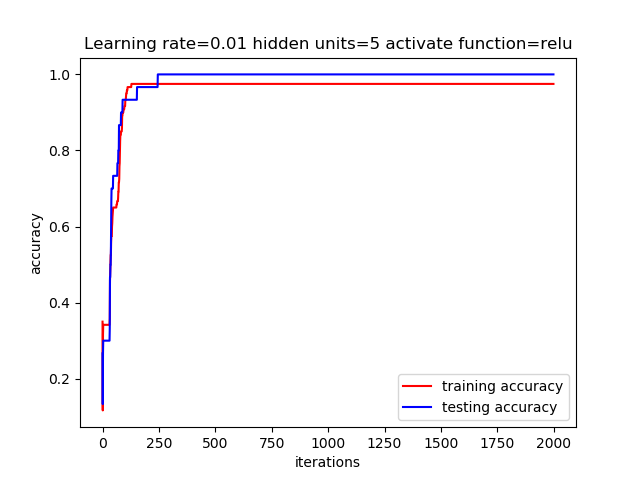
\includegraphics[scale=0.3]{accuracy_relu_5.png} 
    %\caption{fig1} 
    \end{minipage}%  
    \begin{minipage}[t]{0.5\linewidth} 
    \centering 
    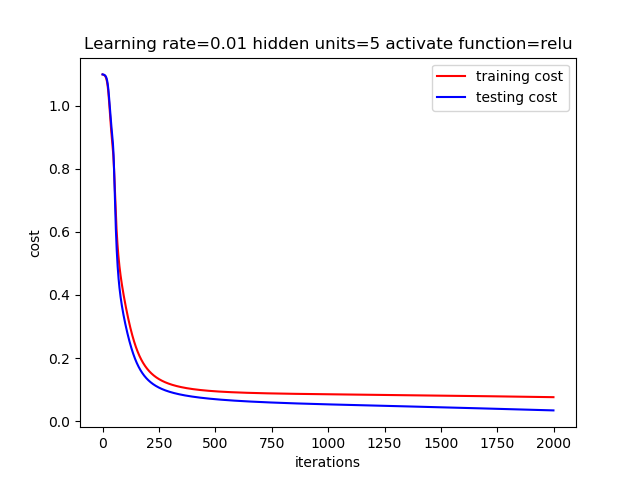
\includegraphics[scale=0.3]{cost_relu_5.png} 
    %\caption{fig2} 
    \end{minipage}% 
    \centering 
    \caption{relu}
    \centering 
    \begin{minipage}[t]{0.5\linewidth}
    \centering 
    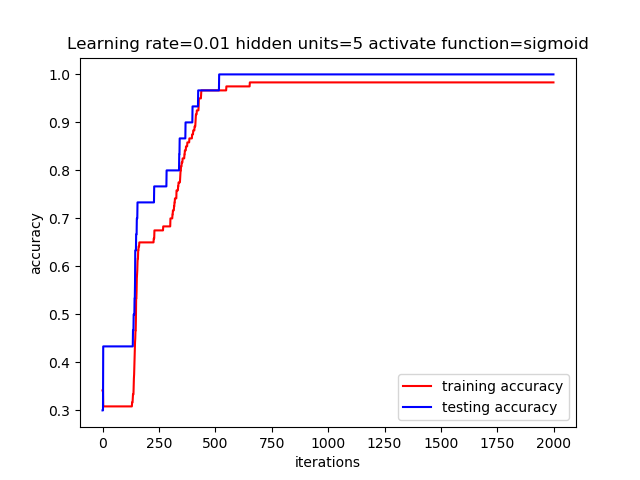
\includegraphics[scale=0.3]{accuracy_sigmoid_5.png} 
    %\caption{fig1} 
    \end{minipage}%  
    \begin{minipage}[t]{0.5\linewidth} 
    \centering 
    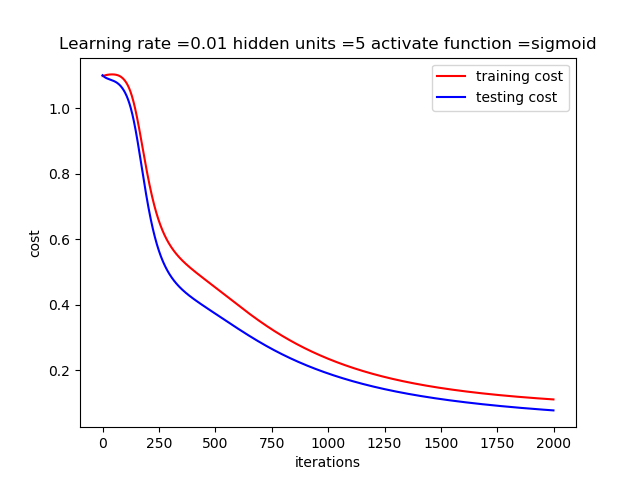
\includegraphics[scale=0.3]{cost_sigmoid_5.png} 
    %\caption{fig2} 
    \end{minipage}% 
    \centering 
    \caption{sigmoid}
    \centering 
    \begin{minipage}[t]{0.5\linewidth}
    \centering 
    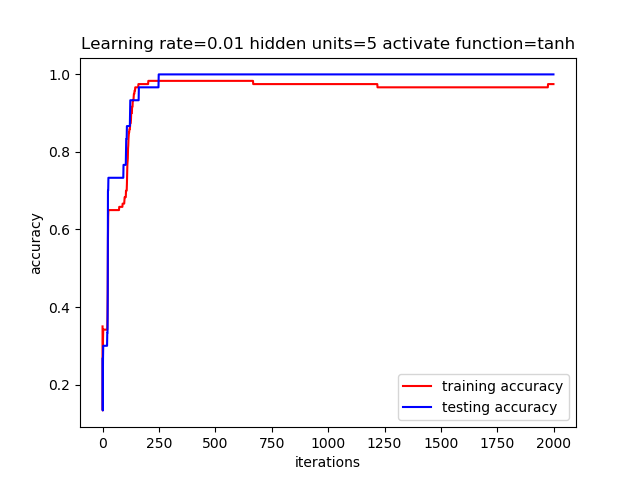
\includegraphics[scale=0.3]{accuracy_tanh_5.png} 
    %\caption{fig1} 
    \end{minipage}%  
    \begin{minipage}[t]{0.5\linewidth} 
    \centering 
    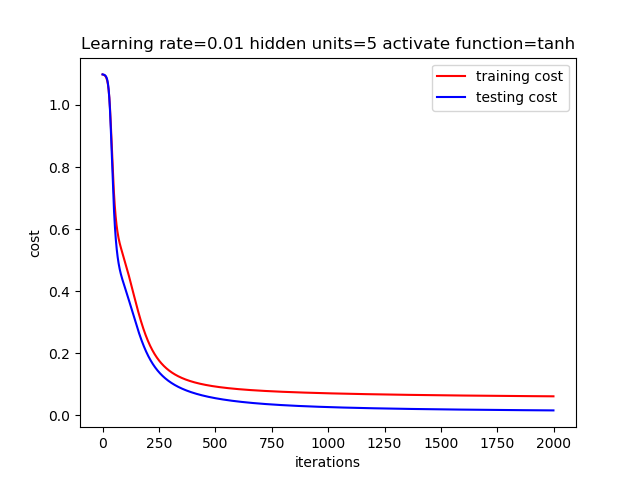
\includegraphics[scale=0.3]{cost_tanh_5.png} 
    %\caption{fig2} 
    \end{minipage}% 
    \centering 
    \caption{tanh} 
\end{figure}

我们可以很明显的发现,使用sigmoid函数后的,损失函数的下降速率明显低于其他两个,而relu和tanh之间,relu又略优于tanh。
在运行速度上(在同一机器),使用relu函数,每训练一轮,要经过1.264ms,而sigmoid和tanh分别为1.424ms和1.475ms,也就是说relu函数的
运算速度要略快于其他两个函数。
\newpage 究其原因,我们可以看看每个函数的数学表达式和函数曲线:\\
\vspace{10pt}
\begin{minipage}[t]{0.3\linewidth}
\centering 
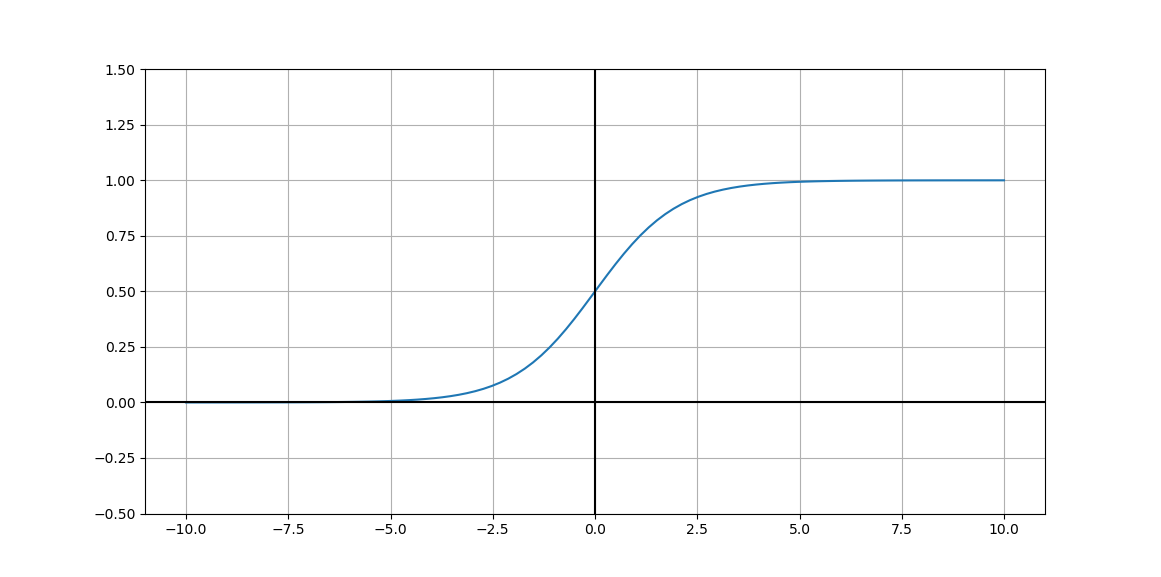
\includegraphics[scale=0.1]{sigmoid.png}     
\end{minipage}%  
\begin{minipage}[t]{0.3\linewidth} 
\centering 
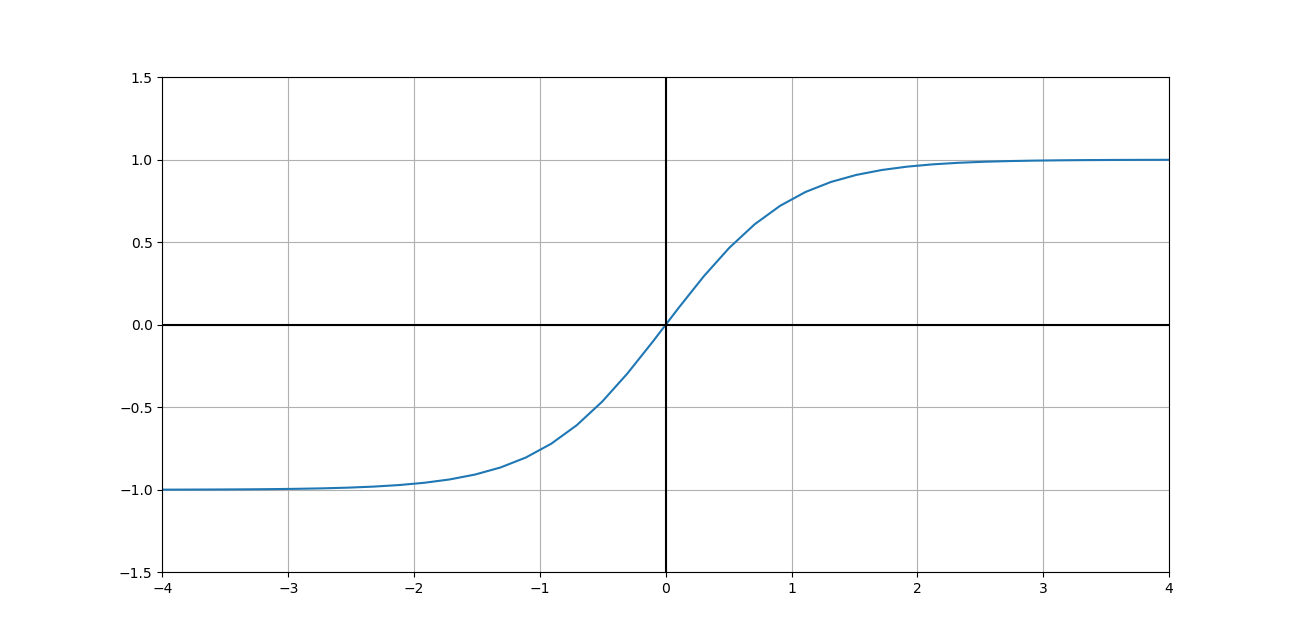
\includegraphics[scale=0.1]{tanh.png} 
\end{minipage}%
\begin{minipage}[t]{0.3\linewidth} 
\centering 
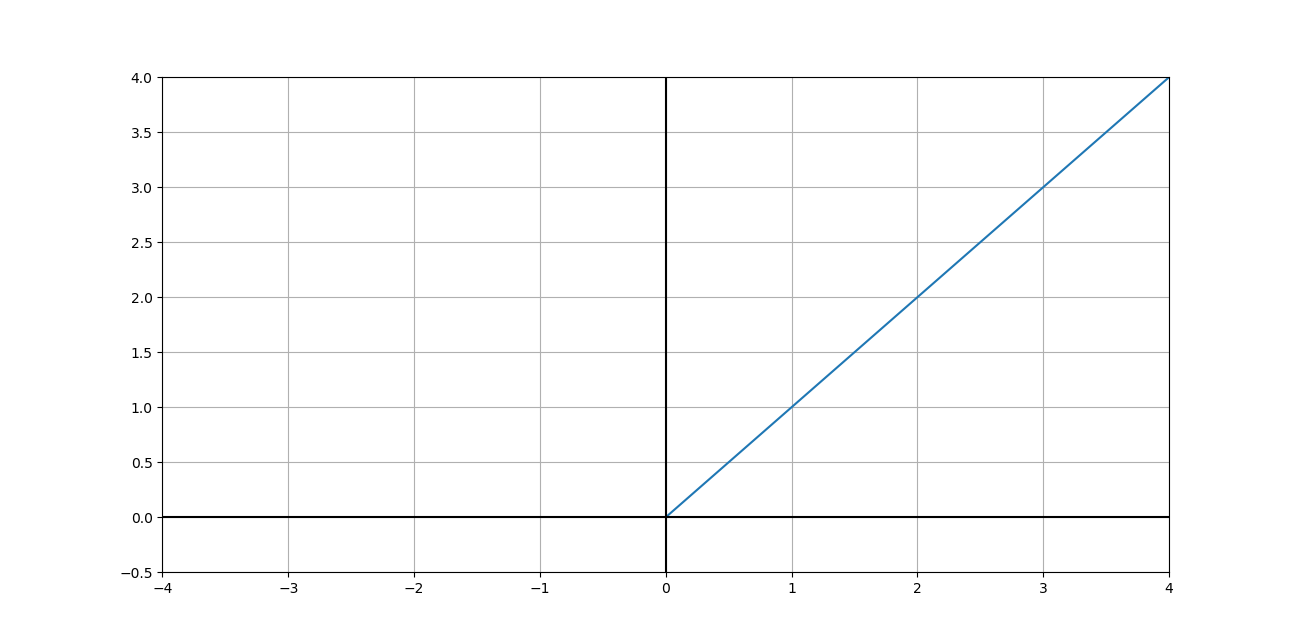
\includegraphics[scale=0.1]{relu.png} 
\end{minipage}\\
\begin{minipage}[t]{0.3\linewidth}
\centering 
$\mathbf{y}=\frac{1}{1+e^{-x}}$
\end{minipage}%  
\begin{minipage}[t]{0.3\linewidth} 
\centering 
$\mathbf{y}=\frac{e^x-e^{-x}}{e^x+e^{-x}}$
\end{minipage}%
\begin{minipage}[t]{0.3\linewidth} 
\centering 
$\mathbf{y}=max(x,0)$
\end{minipage}
\vspace{10pt}

从时间因素来看,tanh和sigmoid函数中包含指数运算,因此不管是正向传播还是
反向传播,都需要进行指数运算,而relu函数都是线性运算,所需的计算时间自然较少。
撇开时间因素不谈,这三个函数还有以下的不同:
\begin{itemize}
    \item[a)] 对于sigmoid函数来说:
    \begin{enumerate}
        \item 在输入很大或者很小的情况下,sigmoid函数的导数值都几乎为0.而反向传播正需要梯度来更新参数,梯度越小,损失函数值自然下降得也越慢。因此如果在对参数进行初始化的时候使参数过大,那么该网络中大多数的神经元都出现了梯度消失的现象,那么损失值的下降将会很慢。
        \item sigmoid函数的函数值是以0.5为中心的。这会导致后层的神经元的输入是非0均值的信号,这会对梯度产生影响:假设后层神经元的输入都为正,那么对w求局部梯度则都为正,
        这样在反向传播的过程中w要么都往正方向更新,要么都往负方向更新,导致有一种捆绑的效果,从而导致梯度下降权重更新时出现 z 字型的下降,使得收敛缓慢。
    \end{enumerate} 
    \item[b)] tanh函数解决了sigmoid函数值不以0为中心的问题,但是梯度消失的问题依然存在
    \item[c)] relu函数的线性和非饱和性很好的解决了梯度消失的问题。但他还有一个很明显的缺点,就是当一个很大的梯度经过一个神经元的时候,
    更新参数之后,导致该神经元以后的梯度都为0,也就是说该神经元的参数停止更新,这将大幅度的降低神经网络的性能。因此学习率的设置就显得尤为重要,合理的学习率会降低这一情况发生的概率 
\end{itemize}
\newpage
\subsection{mnist}
\begin{wrapfigure}{r}{0.3\textwidth}
\vspace{-15pt}
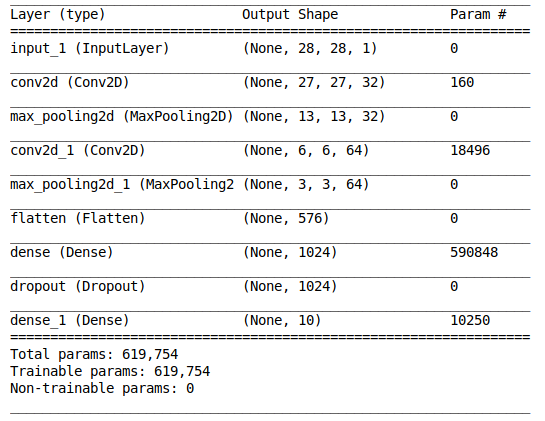
\includegraphics[width=3cm,clip]{CNN.png}\\
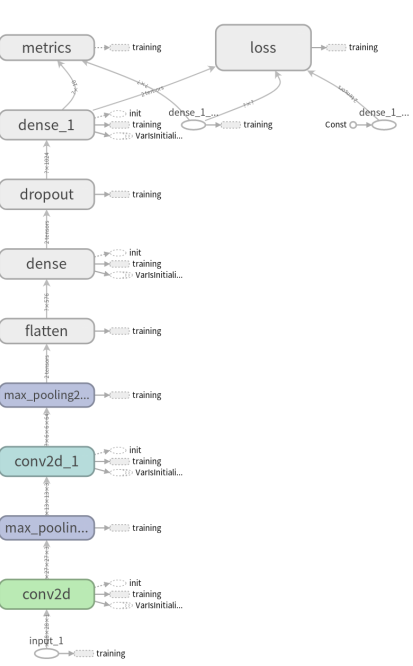
\includegraphics[width=3cm,clip]{CNNnet.png}
\end{wrapfigure}
\par
mnist数据集的数据为70000张大小为28*28的手写数字图片。对于图像处理,使用卷积神经网络最为合适。以下构建CNN网络架构:
\begin{itemize}
    \item 输入层
    \item conv1,含有32个巻积内核,内核大小为(2,2),步长为1,输出大小为(None,27,27,32),激活函数为relu
    \item maxpooling1,内核大小(2,2),步长为2,输出大小为(None,13,13,32)
    \item conv2,含有64个巻积内核,内核大小为(3,3),步长为2,输出大小为(None,6,6,64),激活函数为relu
    \item maxpooling2,内核大小(2,2),步长为2,输出大小为(None,3,3,64)
    \item 全连接层,输出大小为(None,1024),dropout概率为0.6,激活函数为relu
    \item 全连接层,输出大小为(None,10),激活函数为softmax
\end{itemize}

优化方法使用adam优化器,学习率默认0.0001,损失函数使用交叉熵,训练12次测试集准确率大概能达到99.25\%,训练过程中准确率和损失函数值变化情况如下图:
\begin{figure}[htb]
    \centering 
    \begin{minipage}[t]{0.5\linewidth}
    \centering 
    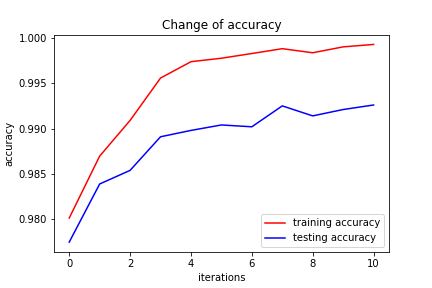
\includegraphics[scale=0.3]{accuracy_mnist.png} 
    %\caption{fig1} 
    \end{minipage}%  
    \begin{minipage}[t]{0.5\linewidth} 
    \centering 
    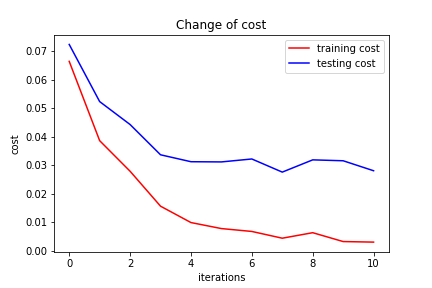
\includegraphics[scale=0.3]{cost_mnist.png} 
    %\caption{fig2} 
    \end{minipage}% 
    \centering 
    \caption{relu} 
\end{figure}
\newpage
\subsection{附加题}
假设预测值为$\mathbf{y}$,真实值为$\mathbf{y}'$,
按要求可得,输入$\mathbf{y}$与输出$\mathbf{x}$的关系为:
\begin{displaymath}
    \mathbf{y}= sigmoid(\mathbf{X}\mathbf{W_1}+\mathbf{b_1})\mathbf{W_2}+\mathbf{b_2}
\end{displaymath}
交叉熵损失函数表达式为:
\begin{displaymath}
    loss = - \sum_i y_i'*log(softmax(y)_i)
\end{displaymath}
设$Z_1=XW_1+b_1,A_1=sigmoid(Z_1),Z_2=A_1W_2+b_2,A_2=softmax(Z_2)$,
由此计算导数:
\begin{eqnarray*}
    \begin{aligned}
    &\frac{\partial loss}{\partial Z_2}=A_2-y'
    &\quad\frac{\partial loss}{\partial W_2}=A_1^T\frac{\partial loss}{\partial Z_2}
    &\quad\frac{\partial loss}{\partial b_2}=\frac{\partial loss}{\partial Z_2}\\
    &\frac{\partial loss}{\partial Z_1}=\frac{\partial loss}{\partial Z_2}W_2^T\odot A1\odot(1-A1)
    &\quad\frac{\partial loss}{\partial W_1}=X^T\frac{\partial loss}{\partial Z_1}
    &\quad\frac{\partial loss}{\partial b_1}=\frac{\partial loss}{\partial Z_1}
    \end{aligned}
\end{eqnarray*}
由以上表达式在代码中构建正向传播和反向传播,完成对损失函数的优化。
以下为优化过程中准确率和损失函数值的变化曲线图:\\
\begin{figure}[htb]
    \centering 
    \begin{minipage}[t]{0.5\linewidth}
    \centering 
    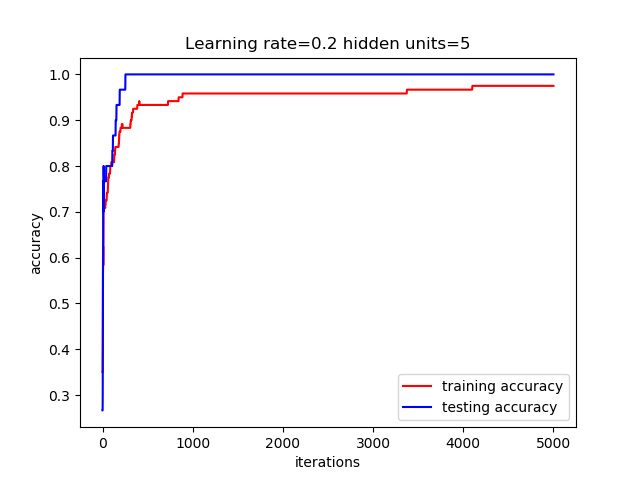
\includegraphics[scale=0.3]{accuracy_5_diy.png} 
    %\caption{fig1} 
    \end{minipage}%  
    \begin{minipage}[t]{0.5\linewidth} 
    \centering 
    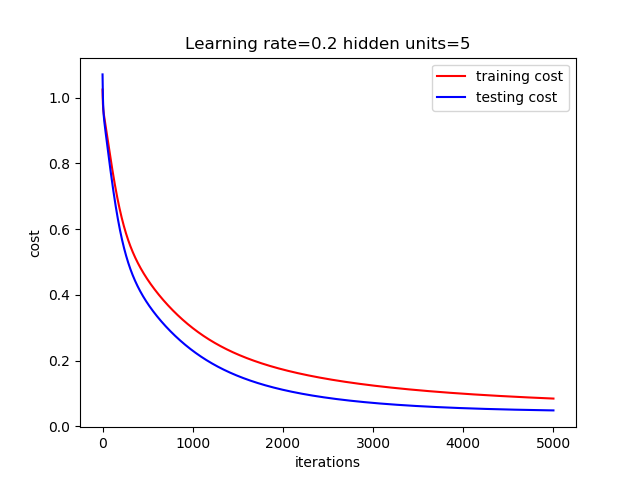
\includegraphics[scale=0.3]{cost_5_diy.png} 
    %\caption{fig2} 
    \end{minipage}%  
\end{figure}
\par
与使用tensorflow框架对比,在性能上来说区别不大,只是相应的最优学习率和训练次数有所差别,最终的结果差别不大。
但明显的发现,使用numpy自行实现的程序的运行速度要比tensorflow快得多(前者0.42ms每步而后者1.424ms)。我认为应该是
原因在于自行实现的程序没有那么多的依赖库,因此节省了很多不必要的时间消耗。而使用tensorflow处理这一数据量较小的数据集,无异于
杀鸡而用牛刀。
\section{总结}
本次作业主要考察的地方有:
\begin{itemize}
    \item 交叉熵损失函数与softmax函数的配合使用计算损失
    \item 机器学习框架的使用
    \item 多层神经网络的构建与不同激活函数的使用
    \item 卷积神经网络的构建
    \item 矩阵求导以及正向传播、反向传播的构建
\end{itemize}
总的来说,本次作业涉及的内容较多,对编程与线性代数均有一定的要求。作业完成期间与同学进行了很多深入的交流,不同的思想之间碰撞出了
不少的火花,收益匪浅。
\end{document}